\begin{table}[t]
\scriptsize 
\centering
\begin{tabular}{p{2cm} p{0.8cm} p{2.1cm} p{1.5cm} }
\toprule
\textbf{Library}						& \textbf{Version}	& \textbf{Category}		& \textbf{Protection} \\ 
\midrule
{Botan~\cite{botan_cryptozoo}}				& {1.10.13}			& {Crypto Libraries}		& - \\
{Crypto++~\cite{cryptopp_cryptozoo}}		& {5.6.4}			& {Crypto Libraries}		& - \\
{Libgcrypt~\cite{libgcrypt_cryptozoo}}		& {1.6.6}			& {Crypto Libraries}		& - \\
{LibSodium~\cite{libsodium_cryptozoo}}		& {1.0.12}			& {Crypto Libraries}		& - \\
{LibTomcrypt~\cite{libtomcrypt_cryptozoo}}	& {1.17}			& {Crypto Libraries}		& - \\
{Nettle~\cite{nettle_cryptozoo}}			& {3.3}				& {Crypto Libraries}		& - \\
\midrule
{GnuTLS~\cite{gnutls_cryptozoo}}			& {3.5.13}			& {SSL/TLS Libraries}		& - \\
{mbedTLS~\cite{mbedtls_cryptozoo}}			& {2.3.0}			& {SSL/TLS Libraries}		& - \\
{OpenSSL~\cite{openssl_cryptozoo}}			& {1.1.0f}			& {SSL/TLS Libraries}		& - \\
{WolfSSL~\cite{wolfssl_cryptozoo}}			& {3.9.10}			& {SSL/TLS Libraries}		& - \\ 
\bottomrule
\toprule
\textbf{Application}					& \textbf{Version}	& \textbf{Category}		& \textbf{Protection} \\ 
\midrule
{7-Zip~\cite{7zip_cryptozoo}}				& {9.20}			& {File Compressor}			& - \\
{Ccrypt~\cite{ccrypt_cryptozoo}}			& {1.10}			& {File Encryptor}			& UPX \\
{Cryptcat~\cite{cryptcat_cryptozoo}}		& {1.2.1}			& {Messenger}				& - \\
{Cryptochief~\cite{cryptochief_cryptozoo}}	& {1.337}			& {File Encryptor}			& - \\
{Enpass~\cite{enpass_cryptozoo}}			& {5.6.0}			& {Password Manager}		& - \\
{Imagine~\cite{imagine_cryptozoo}}			& {1.1.0}			& {Picture Browser}			& UPX \\
{IpMsg~\cite{ipmsg_cryptozoo}}				& {4.60}			& {Messenger}				& - \\
{KeePass~\cite{keepass_cryptozoo}}			& {1.34}			& {Password Manager}		& - \\ 
{MuPDF~\cite{mupdf_cryptozoo}}				& {1.11}			& {PDF Parser}				& - \\
{PSCP~\cite{putty_cryptozoo}}			& {0.62}			& {SSH client}				& - \\
{Sage~\cite{sage_cryptozoo}}				& {2.0}				& {Ransomware}				& - \\
{Ultrasurf~\cite{ultrasurf_cryptozoo}}		& {15.04}			& {Proxy client}			& Themida \\
{WannaCry~\cite{wannacry_cryptozoo}}		& {1.0}				& {Ransomware}				& Dynamic DLL \\
{Wget~\cite{wget_cryptozoo}}				& {1.11.4}			& {Downloader}				& - \\
{WinRAR~\cite{winrar_cryptozoo}}			& {5.40}			& {File Compressor}			& - \\
\bottomrule
\end{tabular}
\vspace{0.1cm}
\caption{The collected binary executables in our benchmark.}\label{tab:cryptozoo}
\end{table}


    \begin{table}[t]
\scriptsize 
\centering

%\vspace{-0.55in}
%\vspace{-0.4in}
\scalebox{1}{
\begin{tabular}{l l c c c c c ccc}

\toprule
\textbf{Target} & \textbf{Algorithm} & \textbf{B1} & \textbf{B2} & \textbf{B3} & \textbf{N} & \textbf{S} & \textbf{IL} \\
\hline 
\multirow{4}{*}{Botan}		& AES-256			& 53 & 13 & 7			& 1 & 240 & 32 \\
							& RSA-2048			& 1180 & 569 & 162		& 6 & 1024 & 256 \\
							& ECDSA	& 958 & 921 & 300		& 2 & 224 & 128 \\
\midrule                            
\multirow{4}{*}{Crypto++}	& AES-256			& 1281 & 26 & 5			& 1 & 240 & 32 \\
							& RSA-2048			& 1949 & 924 & 214		& 6 & 896 & 256 \\
							& ECDSA	& 1916 & 1425 & 305		& 8 & 288 & 64 \\
\midrule
\multirow{4}{*}{Libgcrypt}	& AES-256			& 126 & 25 & 3		& 1 & 240 & 32 \\
							& RSA-2048			& 565 & 463 & 153	& 6 & 896 & 896 \\
							& ECDSA	& 340 & 322 & 49	& 10 & 320 & 96 \\
\midrule
\multirow{2}{*}{LibSodium}	& AES NI-256		& 7 & 4 & 4			& 1 & 240 & 32 \\
							& Ed25519			& 690 & 686 & 171	& 8 & 288 & 256 \\
\midrule
\multirow{4}{*}{LibTomcrypt}	& AES-256			& 60 & 43 & 4		& 1 & 240 & 32 \\
							& RSA-2048			& 404 & 385 & 69	& 7 & 1152 & 1152 \\
							& ECDSA	& 330 & 274 & 72	& 4 & 128 & 97 \\
\midrule
\multirow{4}{*}{Nettle} 	& AES-256				& 38 & 13 & 3		& 1 & 240 & 32 \\
							& RSA-2048				& 411 & 87 & 61		& 6 & 1152 & 896 \\
							& ECDSA		& 186 & 92 & 39		& 8 & 288 & 32 \\
\midrule
\midrule
\multirow{4}{*}{mbedTLS}	& AES-256			& 44 & 40 & 13		& 1 & 240 & 32 \\
							& RSA-2048			& 154 & 138 & 39	& 12 & 1664 & 256 \\
							& ECDSA	& 255 & 245 & 47	& 9 & 384 & 64 \\
\midrule
\multirow{4}{*}{OpenSSL}	& AES-256			& 58 & 10 & 4		& 1 & 240 & 32 \\
							& RSA-2048			& 210 & 175 & 41	& 10 & 1552 & 640 \\
							& ECDSA	& 188 & 143 & 17	& 6 & 192 & 50 \\
\midrule
\multirow{4}{*}{WolfSSL}	& AES-256			& 50 & 36 & 4		& 1 & 240 & 32 \\
							& RSA-2048			& 295 & 235 & 36	& 7 & 1152 & 1152 \\
							& ECDSA	& 277 & 202 & 27	& 5 & 160 & 32 \\
\midrule
\midrule
7-zip						& AES NI-256		& 2 & 2 & 2	 		& 1 & 240	& 32 \\
\midrule
Ccrypt 						& AES-256			& 44 & 5 & 1	 	& 1 & 240	& 32 \\
\midrule
Cryptcat					& Twofish			& 54 & 14 & 7		& 1 & 160	& varied \\
\midrule
Cryptochief 				& Proprietary $\ast$	& 23 & 12 & 1		& 1 & 8		& 3 \\
\midrule
Enpass 						& AES NI-256		& 8 & 3 & 3	 		& 1 & 240	& 32 \\
\midrule
Imagine						& DSA-1024 $\ast$	& 241 & 72 & 12	 	& 5 & 464	& 928 \\ % should be 464 == 128*3 + 40*2!!!
\midrule
IpMsg						& AES-256			& 168 & 12 & 4		& 1 & 240	& 32 \\
\midrule
Keepass						& AES-256			& 481 & 118 & 19	& 1 & 240 & 32 \\
\midrule
MuPDF						& AES-128			& 262 & 46 & 4	 	& 1 & 176	& 16 \\
\midrule
PSCP						& AES-256			& 195 & 9 & 5		& 1 & 240	&  32 \\
\midrule
Sage						& ChaCha20 $\ast$	& 31 & 17 & 2		& 1 & 256	& 32 \\
\midrule
UltraSurf					& RC4 $\ast$		& 191 & 79 & 6		& 1 & 1024 & 16 \\
\midrule
WannaCry					& AES-128 $\ast$	& 26 & 12 & 3	 	& 1 & 352	& 16 \\
\midrule
Wget						& AES-256			& 268 & 22 & 3		& 1 & 240	& 32 \\
\midrule
\multirow{2}{*}{WinRAR} 	& AES-128 $\ast$	& 181 & 58 & 3		& 1 & 176	& 32 \\
 							& AES-256 $\ast$	& 214 & 51 & 3	 	& 1 & 240	& 48 \\
\bottomrule


% \multicolumn{7}{p{8.4cm}}{B1: the number of basic blocks, each of which contains certain ratio (0.15) of data arithmetic instructions and memory I/O instructions}\\
% \multicolumn{7}{p{8.4cm}}{B2: the number of basic blocks, each of which belongs to B1 and also has a linear relation with the input size}\\
% \multicolumn{7}{p{8.4cm}}{B3: the number of basic blocks, each of which belongs to B2 and also contains data bundles with high entropy and randomness}\\
% \multicolumn{7}{p{8.4cm}}{ S: the size of the identified key buffer}\\
% \multicolumn{7}{p{8.4cm}}{IL: the input length of the identify key buffer}\\
 
% \multicolumn{8}{p{8.5cm}}{\textbf{B1}: the number of basic blocks, each of which contains the data arithmetic instructions; \textbf{B2}: the number of basic blocks, each of which belongs to B1 and also has a linear relation with the input size; \textbf{B3}: the number of basic blocks, each of which belongs to B2 and also contains data bundles with high entropy and randomness; \textbf{N}: the number of the identified key buffer(s); \textbf{S}: total size of the identified key buffer(s); \textbf{IL}: the input length of the identify key buffer(s).}
 
\end{tabular}
}
\caption{Results of the key pinpointing and key identification. $\ast$ denotes that the implementation of this algorithm is proprietary.% for our benchmark suite. % In the experiments we mainly chose AES-256, RSA-2048, DSA-2048, and ECDSA-secp256k1. For Libsodium, we choose AES-128 and Ed25519. The definitions of abbreviation in heading are: B1/B2/B3 denotes the number of remained code blocks after the filtering of data arithmetic instruction testing, number of execution, and entropy/randomness in turn, SoKB denotes the size of the key buffer in byte.
}\label{tab:lib_results}
\end{table}
    
We have tested \sysname with {10 popular crypto libraries and 15 real-world programs}, identifying many insecure keys among these programs. In this section, we present our evaluation results. We first describe our experimental setup in \S\ref{sec:eval:setting}, then present the detection results for crypto keys in \S\ref{sec:eval:results}, and finally detail the identified insecure keys in \S\ref{ss:insecurekey}. 

\subsection{Experiment Setup}\label{sec:eval:setting}

%\paragraph{Benchmark Collection} 
% While there are efforts of analyzing the crypto software (e.g., CryptoHunt~\cite{xu2017cryptographic}), 
As far we know, there are no standard benchmarks that cover widely used crypto algorithms. 
As such, we create a benchmark, detailed in~\autoref{tab:cryptozoo}, that contains recent versions of 10 crypto libraries and 15 real-world programs that use crypto operations. 
%We used the latest stable version of each library or program as of September 1, 2017.
Our collected benchmark suite includes:
(a) popular standard symmetric ciphers (AES, Twofish), asymmetric ciphers (RSA), stream ciphers (RC4, ChaCha20), and digital signatures (DSA, ECDSA, Ed25519);
(b) different key sizes for the same algorithm (e.g., AES-128, AES-256); 
(c) one proprietary cipher (Cryptochief); 
(d) proprietary programs for which we do not have access to the source code (Cryptochief, Imagine,  UltraSurf, WinRAR); 
(e) benign programs that use binary code protection techniques such as code packing (Ccrypt, Imagine, UltraSurf); and 
(f) two samples from recent ransomware families (Sage, WannaCry).

For each crypto library, we developed test programs to encrypt/decrypt using  \textsf{\small AES, RSA}, and to sign/verify using \textsf{\small  ECDSA}. Since \textsf{\small Libsodium} does not support \textsf{\small RSA} and \textsf{\small ECDSA}, we included the \textsf{\small Ed25519} digital signature instead.

For each program, we have manually built the ground truth regarding their key management using the program's source code (when available), or by manually reverse-engineering the executables (for proprietary programs and malware). 
Note that for programs for which source code is available, we only use the source code to build the ground truth. 
\sysname operates on executables and does not require access to the program's source or debugging symbols.

\paragraph{Input Preparation} %Since \sysname is a dynamic analysis tool, we have to execute it with proper test cases. 
We  have prepared test cases of different sizes for each program, so that each test case triggers a cryptographic operation.
The test cases can be easily produced using the high-level descriptions of the software available on their webpages, 
e.g., that it encrypts a file with password, 
there is no need to know any low level details about the program. 
Furthermore, most of the payload of the test cases can be random, as long as the crypto operation is triggered.  
For the differential analysis, we also prepared test cases of different sizes that do not trigger a crypto operation. 
%For instance, we prepared for two files of different size (10K and 100K) for the HTTPS downloading test of \textsf{\small Wget} to measure the variation of two executions. 
% For instance, for \textsf{\small Ultrasurf} that communicates with a remote server and the content is encrypted by its internal crypto scheme, we just need to prepare for a test case with common message that definitely triggers the communication (and thus the encryption).

\paragraph{Executions} 
For each test case, \sysname executes the program three times with different instrumentations. 
In the first execution, \sysname obtains basic block statistics to identify candidate crypto basic operation blocks. 
In the second execution, \sysname tests the data randomness to identify the actual crypto basic blocks and analyzes them to locate the crypto keys. 
In the third execution, \sysname performs the taint analysis of the crypto keys to detect insecure crypto keys.
   
\paragraph{Host} 
\sysname can run on both Windows and Linux thanks to Pin's support for both platforms. 
We use a Dell workstation installed with both Windows 7 and Fedora 25 operating systems as the testing platform. 
The workstation has an Intel Core i7-6700 CPU (3.4GHz), with 16GB physical memory and a 2TB disk. \looseness=-1


\subsection{Effectivenesses of Key Identification}\label{sec:eval:results}

\autoref{tab:lib_results} details the results of \sysname's key buffer pinpointing for each of the programs\footnote{Note that \textsf{\small GnuTLS} is missing because it relies on \textsf{\small Nettle} or \textsf{\small Libgcrypt} as its crypto backend, and the results of both \textsf{\small Nettle} and \textsf{\small Libgcrypt} are already listed.}. 
The table shows in column \textbf{B1} the number of candidate basic blocks that contain a high arithmetic instruction ratio; in \textbf{B2} the subset of B1 candidate basic blocks with a linear relation with the input size; in \textbf{B3} the number of identified crypto basic blocks, i.e., B2 candidate basic blocks that produce data bundles with high randomness; in \textbf{N} the number of identified key buffers; in \textbf{S} the total size of the identified key buffers; and in \textbf{IL} the input length of the identified key buffers.

We can observe from columns \textbf{B1}--\textbf{B3} that all three constraints to identify crypto basic blocks are needed.
If we only use the first constraint, i.e., arithmetic instruction ratio, many irrelevant basic blocks are included especially for data transformation programs (e.g., \textsf{\small WinRAR, MuPDF}). 
If we only use the first two constraints, asymmetric ciphers still have a large number of candidate basic blocks. 
Thus, we must also the randomness of the operated data to locate the crypto basic blocks that actually use the crypto key. 

We evaluate the correctness of the crypto key detection using the manually-generated ground truth. 
We do not find any false positives among these programs, but false positives are possible in some cases discussed in  \S\ref{sec:discussion}, 
e.g., if keys are stored in registers.
We find two false negatives, one in  \textsf{\small Wget}, the other in \textsf{\small PSCP}. Both are due to key exchange protocols that combine an asymmetric cipher with a symmetric cipher. 
In both cases, \sysname only discovers the secret key of the symmetric cipher because there is a linear relation between the number of crypto basic block executions and the input size. Since the input for the asymmetric cipher is a single block when protecting the symmetric key, \sysname is not able to pinpoint the public keys. However, if the public key is used to protect the data rather than the key % or sign multiple messages, 
our analysis is able to identify these public keys (e.g., the case of \textsf{\small Imagine} discussed in \S\ref{ss:insecurekey}). 
%
% {Fortunately, the false negatives wit public key cryptosystem does not weaken the effectiveness of our analysis. Since the sole purpose of the public key is to protect the symmetric key, \sysname focuses on the symmetric key.
% For instance, the detection of insecurely generated key treats the public key as normal data but is still able to find the problem: the buffer of public key does not contains two tags.
% Moreover, if a public-key cryptosystem is used to protect the data rather than the key, our analysis is still available (e.g., the case of \textsf{\small Imagine}).}

To better understand how our analysis performs, we have conducted an in-depth investigation and obtained a number of interesting findings, which are summarized below:%\begin{enumerate}[label=(\Roman*)]
%\begin{compactitem}%[label=(\roman*)]

%\item
\paragraph{Key buffers of block ciphers}
In our benchmark the most frequently used cipher is the \textsf{\small AES} block cipher.
We found that all of the \textsf{\small AES} implementations store the round keys (11 or 15 rounds) in one key buffer (176 or 240 bytes).
Nonetheless, the format of those key buffers are often diversified in terms of byte orders and buffer sizes.
For instance, \textsf{\small AES} key buffers of \textsf{\small WinRAR} and \textsf{\small Putty-SCP} use different byte orders. Meanwhile, malware authors can also deliberately obfuscate the key format to evade the detection. We found that the recent ransomware, \textsf{\small WannaCry},  allocates a non-standard \textsf{\small AES-128} round key buffer with double the normal size (i.e., 352 instead of 176 bytes). 
As a result, signature-based key searching techniques (e.g., ~\cite{shamir1999playing, maartmann2009persistence, aeskeyfind_debian}) are unlikely to identify the key. 
\sysname instead is not affected by such an implementation variation. %since \sysname does not rely on any assumption of memory layout of the key and it identifies the key buffer as a data bundle in program despite its format. 
Additionally, \sysname handled Intel's hardware \textsf{\small AES} encryption in the case of \textsf{\small Libsodium}, \textsf{\small Enpass}, and \textsf{\small 7-zip} through directly labeling \textsf{\small AES NI} instructions and identifying the relevant key buffers.
% \sysname also detected the key buffer of \textsf{\small Twofish} block cipher in \textsf{\small Cryptcat} and we found the input length of this cipher is varied according to different user inputs.

\paragraph{Key buffers of stream ciphers}
In our benchmark three programs (\textsf{\small Cryptochief, Ultrasurf}, and \textsf{\small Sage}) use stream ciphers.
A stream cipher often maintains a ``state'' in a fixed-length memory buffer to update the key stream. 
This state is continuously updated during the encryption.
Therefore we could not distinguish it by simply assuming the key is immutable.
\sysname pinpoints the key buffer from crypto blocks that operate on it, and accurately detects its range.
The key buffers of stream ciphers \textsf{\small RC4} and \textsf{\small ChaCha20} are both 256 bytes and the home-made stream cipher in \textsf{\small Cryptochief}~\cite{cryptochief_cryptozoo} uses a 8-byte key buffer, as shown in the \textbf{S}-column.

\paragraph{Key buffers of public-key ciphers} 
Unlike block ciphers and stream ciphers where \sysname identifies a single buffer (\textbf{N} column in \autoref{tab:lib_results}), 
 \sysname identified multiple key buffers for asymmetric ciphers.
This happens because public keys used by asymmetric ciphers usually consists of several components that may be stored in different buffers, 
e.g., $d$ and $n$ in \textsf{\small RSA}. % as two 2048-bit integers. 
%A large integer is usually stored using a large integer \texttt{struct}. % which keeps data size and a pointer of a continuously allocated array. 
%The public key cipher takes such structs as parameters, and the core calculation with the arithmetic operations (e.g., a series of multiplication and modular calculations) produces highly random data.  Through analyzing the core code blocks, our key identification algorithm directly detects the crypto code blocks and then classifies key in allocated array of the large integers. That explains why we found several key buffers for each public-key cipher.
%
%In every crypto libraries we tested and also the application \textsf{\small Imagine}, \sysname detected the key of public-key ciphers as a set of buffers. 
%We then manually verified them and confirmed that they are actually large integer structs storing public and private keys.
%Since \sysname dose not have the knowledge of each element of the key in those detected arrays, it only considered them as an integrated key. % In the S-column, we reported the total length of all classified key buffers.
%\ZQ{In Imagine, there are five large integers as described later. Here the buffer is only 456 bytes. How do you justify that? How many buffers you found? The S column means which key in Imagine? Also, note that for public key crypto, there are usually multiple Keys. How do you capture that in your presented table?} 
Interestingly, we found the length of key buffers are often much larger than the length of the required public key. 
We then checked the source code of each crypto library and found that certain public key encryption are actually implemented in a very optimized way, which often uses a varied public key with larger integers. 
For instance, we found all tested crypto libraries implement the \textsf{\small RSA} algorithm with the Chinese Remainder Theorem (CRT) optimization, which requires a number of extra parameters (e.g., $d_p$, $d_q$, $q_{inv}$) besides the well-known parameters (e.g., $n$, $d$, $p$, $q$). 
In this situation the detected \textsf{\small RSA} key buffers covers all used large integers.

%\JR{Note that \sysname only detects public-key buffers if the public-key cipher is executed multiple times. If a public-key cipher is only used for a fixed times (e.g., in key negotiations of \textsf{\small Wget} and \textsf{\small Putty-SCP}, the public-key buffers are not detected}.
%The situation of \textsf{\small ECDSA} key is similar since it contains the used elliptic curve with several parameters. That is why the number of public key buffers identified by \sysname is larger than what a typical public key crypto would need. Also, very interestingly, even for the same cipher (\textsf{\small RSA-2048} or \textsf{\small ECDSA}), the detected key varies in number of buffers. That is because each crypto library defines its own key struct with different number of data members. Also, the \textsf{\small DSA} key used in \textsf{\small Imagine} contain five parameters ($p$, $q$, $g$, $y$, $k$) and \sysname detected all of them. \looseness=-1

% \ZQ{Does CRT optimization has an example in the table?}
%four large integer arithmetics functions $mod$, $mod\_inv$, $pow$, and $mul\_mod$ to fulfill the public key signature verification. Hence, the public key signature verification is not implemented as an independent function but as a part of a registration authorization function. If the detection needs to recognize the algorithm and relevant parameters, it will suffer from issues such as function boundary identification and data type inference. In comparison, \sysname is straightforward to identify the actually used public key buffer in these operations.

%Notice that some public keys are used as subordinate keys in the execution of Wget, Putty-SCP, and Ultrasurf. This situation is out of this paper's scope and  is ignored as discussed in Section~\ref{ss:overview}.
%\end{compactitem}


\subsection{Effectiveness of Insecure Key Detection}
\label{ss:insecurekey}


%%%%%%%%%%%%%%%%%%%%%%%%%%%%%%%%%%%%%%%%%%%%%%%%%%%%%%%%%%%%%%%%%%%%%%%%%%%%%%%%%%%%%%%%%%%%%%%%%%%%%%%%%%%%%%%%%%%%%%%%%%%%%%%%5


\begin{table}[t]
\scriptsize
\centering

\begin{tabular}{l | c| c |c |c | c | c }
\toprule
 			&  &  & \multicolumn{4}{c}{{\bf RK}} \\
\cline{4-7}
{\bf Target}	& {\bf DGK}  & {\bf INK} & {\bf NMZ} & {\bf MMZ} & {\bf RKPS} & {\bf RKPH} \\
\hline\hline
Botan		            & -  & - & - & - & - & - \\
Crypto++            & -  & - & - & - & - & - \\
Libgcrypt		    & -  & -  & -  & \Y & -  & - \\
LibSodium		 & -  & - & \Y	& - &- & -\\ 
LibTomcrypt		& -  & - & \Y	& -	& - & -\\
Nettle			          & - & -  & \Y &  - & -  & - \\
\hline
GnuTLS			     & - & - & - & \Y 	& -  & - \\
mbedTLS			  & - & - & - & \Y 	& -  & - \\
OpenSSL			   & - & - & - & \Y & -  & - \\
WolfSSL			     & - & - & \Y & -	& -  & - \\
\hline\hline
7-zip			           & - 	& - & - & - & \Y & - \\
Ccrypt			         & - & - & - & - & - & \Y	\\
Cryptcat		       & - & - & - & -	& - & \Y	\\
Cryptochief		   & \Y	& - & - & - & - & \Y	\\
Enpass			        & -	& - & - & - & \Y & - \\
Imagine			       & \Y	& - & - & - & - & - \\
IpMsg			         & - & \Y & - & - & \Y & - \\
Keepass			     & - & - & -  & - & \Y & - \\
MuPDF			      & -	& - & - & - & \Y & - \\
PSCP		            & -  & - & - & - & - & - \\
Sage			          & - & - & - & - & \Y & - \\                                            
UltraSurf		     & - & \Y & - & - & \Y & - \\
WannaCry		  & - & - & - & - & \Y & - \\
Wget			          & - & - & - & - & \Y & - \\
WinRAR			      & - & - & - & - & - & \Y	\\
\bottomrule
\end{tabular}

\caption{Results of the detected insecure keys in the tested benchmarks.}\label{tab:insecKey}
\end{table}

After pinpointing the crypto keys, \sysname uses the key tracking Pintool to identify  insecure keys: deterministically generated keys (DGK), insecurely negotiated keys (INK), and recoverable keys (RK). \autoref{tab:insecKey} summarizes the detection results. Among the 25 tested programs, 22 contain at least one insecure key. Only three (\textsf{\small Botan}, \textsf{\small Crypto++}, \textsf{\small PSCP}) do not have any insecure crypto keys. Overall, \sysname finds 25 insecure keys in 8 libraries and 14 applications.
Thus, insecure keys occur not only in applications using crypto operations, but also in well-established crypto libraries.

The most common class of identified insecure keys are recoverable keys. 
\sysname found 21 recoverable keys in 8 libraries and  13 applications. 
\sysname also found two deterministic keys (each in a separate application) and two insecurely negotiated keys (each in a separate application as well).
%
In the following, we detail the detection of each class of insecure keys.

\paragraph{\bf{(I) Detecting DGK}}\label{sec:eval:keygen}
Since the key generation process is not managed by the crypto libraries, we excluded the libraries from the detection of deterministically generated keys, and only evaluated the 15 applications. 
Among the 15 applications, \sysname identified deterministically generated keys in two: \textsf{\small Cryptochief} that uses a proprietary stream cipher and \textsf{\small Imagine} that uses a close-source implementation of DSA-1024.

%\paragraph{Hardcoded Crypto Key}
The first case of DGK is in the  \textsf{\small Imagine} picture browser software, which uses a digital signature to verify whether a user provided license code is valid.
%\sysname first found that the basic blocks for license code verification contain a high ratio of arithmetic instructions.
%Then we provided the program with multiple (invalid) license codes to check the number of execution and the variation of used memory buffers.
\sysname identified five crypto key buffers. Those buffers had only deterministic taint tag, which indicated a deterministic key is used.
We then conducted a manual analysis of the application and found a very complex crypto flaw:
	the program uses an incorrect \textsf{\small DSA} signature verification to check the license code,
    which leads to the exposure of private key.
Such an insecure key management has actually been leveraged to break the \textsf{\small ECDSA} digital signature of Sony Play Station 3~\cite{ecdsa2010ps3}. %The detailed study of why the use of  \textsf{\small DSA} in \textsf{\small Imagine} is insecure and how to leverage it is described in the following.

In particular, a \textsf{\small DSA} cipher contains five large integers:  $p$, $q$, $g$ as fixed parameters (which are public known), 
	$x$ as the private key (which should never be leaked), and $k$ as a random factor (which should be a random secret). 
It generates a public key $y$ = $g^x$ mod $p$. To use \textsf{\small DSA} for digital signature, it has to go through the following two processes.

\begin{compactitem}
\item \textbf{Signature Generation}. To sign a message $m$, the \textsf{\small DSA} cipher computes the signature as a pair ($r$, $s$) with a cryptographic hash function $H$ (e.g., SHA-256) through equation (1) and (2), and then distribute $r$ and $s$ to the receiver.

\begin{equation}
r = g^k \;\; mod \;\; p \;\; mod \;\; q  
\end{equation}

\begin{equation}
s = k^{-1} (H(m) + x \cdot r) \;\; mod \;\; q
\end{equation}

\item \textbf{Signature Verification}.
The receiver then verifies the signature ($r$, $s$) with the public knowledge of $p$, $q$, $g$, $y$ and $H(m)$ to verify whether the signature is valid if $v$, calculated using the following equation from (3) to (6), equals to $r$.

\begin{equation}
w = s^{-1} \; mod \; q
\end{equation}

\begin{equation}
u_1 = H(m) \cdot w \; mod \; q
\end{equation}

\begin{equation}
u_2 = r \cdot w \; mod \; q
\end{equation}

\begin{equation}
v = (g^{u_1} \cdot y^{u_2} \; mod \; p ) \; mod \; q
\end{equation}
\end{compactitem}

Through manual reverse-engineering, we noticed that the five detected key buffers correspond to the publicly known parameters $p$, $q$, $g$, $y$, and the random secret factor $k$. 
Thus, \textsf{\small Imagine} actually leaks the random secret factor $k$ by hard-coding it in the software.
A further reverse engineering of the license registration process of \textsf{\small Imagine} reveals that this software only tells the user $s$ without passing $r$, when a user provides a message $m$ to generate its digital signature. However, the signature verification requires $r$ in equation (5). Therefore, the software then locally computes $r$ by using equation (1) through a hard-coded $k$. 
Unfortunately, the exposure of $k$ is a severe mistake for \textsf{\small DSA} digital signature.
%, and such insecure key management has been leveraged to break the \textsf{\small ECDSA} digital signature of Sony Play Station 3~\cite{ecdsa2010ps3}. 
Specifically, if an attacker has obtained a legal pair of (\emph{r}, \emph{s}), with the leaked $k$, it can then compute the private key $x$ with the following equation:

\begin{equation}
x = r^{-1}(k \cdot s - H(m)) \; mod \; q
\end{equation}

\noindent As such, an attacker is able to forge any other legitimate digital signatures with the private key $x$. We have informed the developer of \textsf{\small Imagine}, and this vulnerability has been confirmed and the patch is still under development as the time of this writing.


%in the Appendix. We have informed the developer of \textsf{\small Imagine}, and this vulnerability has been confirmed and the patch is still under development as the time of this writing.


% In particular, a \textsf{\small DSA} cipher contains five large integers:  $p$, $q$, $g$ as fixed parameters (which are public known),  $x$ as the private key (which should never be leaked), and $k$ as a random factor (which should be a random secret). It generates a public key $y$ = $g^x$ mod $p$. To use \textsf{\small DSA} for digital signature, it has to go through the following two processes.

% \begin{compactitem}
% \item \textbf{Signature Generation}. To sign a message $m$, the \textsf{\small DSA} cipher computes the signature as a pair ($r$, $s$) with a cryptographic hash function $H$ (e.g., SHA-256) through equation (1) and (2), and then distribute $r$ and $s$ to the receiver.

% \begin{equation}
% r = g^k \;\; mod \;\; p \;\; mod \;\; q  
% \end{equation}

% \begin{equation}
% s = k^{-1} (H(m) + x \cdot r) \;\; mod \;\; q
% \end{equation}

% \item \textbf{Signature Verification}.
% The receiver then verifies the signature ($r$, $s$) with the public knowledge of $p$, $q$, $g$, $y$ and $H(m)$ to verify whether the signature is valid if $v$, calculated using the following equation from (3) to (6), equals to $r$.

% \begin{equation}
% w = s^{-1} \; mod \; q
% \end{equation}

% \begin{equation}
% u_1 = H(m) \cdot w \; mod \; q
% \end{equation}

% \begin{equation}
% u_2 = r \cdot w \; mod \; q
% \end{equation}

% \begin{equation}
% v = (g^{u_1} \cdot y^{u_2} \; mod \; p ) \; mod \; q
% \end{equation}

% \end{compactitem}


% Interestingly, \sysname monitored the license registration process of \textsf{\small Imagine}, and identified five memory buffers as key buffers, and reported only deterministic taint tag in the used key buffers, which indicated a deterministic key is used.
% Through manual reverse-engineering of this program, we noticed the five detected key buffers are corresponding to the public known parameters $p$, $q$, $g$, $y$, and the random secret factor $k$. 
% It is very interesting that \textsf{\small Imagine} actually leaks $k$ by making $k$ hard-coded in the software.


% A further reverse engineering of the license registration process of \textsf{\small Imagine} reveals that this software only tells the user $s$ without passing $r$, when a user provides a message $m$ to generate its digital signature. However, the signature verification requires $r$ in equation (5). Therefore, the software then locally computes $r$ by using equation (1) through a hardcoded $k$. 
% Unfortunately, the exposure of $k$ is a severe mistake for \textsf{\small DSA} digital signature, and such insecure key management has been leveraged to break the \textsf{\small ECDSA} digital signature of Sony Play Station 3~\cite{ecdsa2010ps3}. Specifically, if an attacker has obtained a legal pair of (\emph{r}, \emph{s}), with the leaked $k$, she can then compute the private key $x$ with the following equation:

% \begin{equation}
% x = r^{-1}(k \cdot s - H(m)) \; mod \; q
% \end{equation}

%\noindent As such, an attacker is able to forge any other legitimate digital signatures with the private key $x$. We have informed the developer of \textsf{\small Imagine}, and this vulnerability has been confirmed and the patch is still under development as the time of this writing.


%\paragraph{Insufficient Input Length} 
The second case of deterministically generated key was found in \textsf{\small Cryptochief}, a file encryption tool\footnote{Cryptochief was first mentioned by Bruce Schneier in his blog article~\cite{krypto} in 2006. The source code of this program is released~\cite{cryptochief_cryptozoo} after the \emph{Hack.lu} 2014 CTF contest.}. This program accepts two files as inputs: one is a key file and the other is a plaintext file. It then outputs an encrypted file. The lengths of the key and plaintext files are both arbitrary, while the length of the encrypted file is equal to that of the plaintext file.

We used \sysname to monitor the encryption process of \textsf{\small Cryptochief}. Interestingly, \sysname pinpointed that the key buffer has only 8 bytes, and this key buffer is composed from three local input sources.  The IL for each input source is only one byte. 
Therefore, this key buffer has only three bytes IL. This indicates that the key buffer only acquires at most 24-bits of information from the local input. As such, an attacker can easily brute force all the possible keys with just $2^{24}$ possibilities to decrypt any ciphertext without the key file. Our further analysis with program source code reveals that the key derivation function of \textsf{\small Cryptochief} only uses \emph{the head byte, the tail byte and the count of all bytes} of the key  file data to generate an 8-byte key buffer.


\paragraph{{\bf (II) Detecting INK}}\label{sec:eval:keyagaree}
In secure key agreement protocols, the shared key should be influenced by all participants. 
As a result, when \sysname reveals that a shared key is generated with non-deterministic inputs, it further checks whether the non-deterministic inputs come from different parties. 
In our experiments we only consider the client-server model, which involves two participants. 
Of the five crypto protocols in \textsf{\small Cryptcat, Wget, UltraSurf, IpMsg, and PSCP}, two protocols in \textsf{\small Ultrasurf} and \textsf{\small IpMsg} use insecurely negotiated keys. 
Both programs generate session keys locally and the server just accepts the key from the client. 

% Take the \textsf{\small IpMsg} as an example. It is a popular de-centralized instant messenger~\cite{ipmsg_cryptozoo} mainly used for serverless message communication. 
% It claims to support strong message encryption with \textsf{\small RSA-2048} and \textsf{\small AES-256}. 
% \sysname pinpointed a $16 * 15$ bytes key buffer that is only influenced by a local random number generator, thereby leading to an insecurely negotiated key.
% We then manually verified this discovery with the source code of \textsf{\small IpMsg}, and we found the key derivation is very simple. 
{
More specifically, in the case of \textsf{\small IpMsg} that adopts a message encryption with \textsf{\small RSA-2048} and \textsf{\small AES-256}, although \sysname does not identify the used RSA key, it does discovers that the AES key is selected locally (the key is generated using the Windows \texttt{CryptGenRandom} API).
Actually, it is a common mistake to conduct a session key exchange if the client encrypts the session key with a deterministic server RSA public key (and then sends it to the server). 
This not only brings the issue that the session can be controlled by a malicious or tampered client, but also hinders the server to authenticate the client since every attacker could forge the identity through using the public key.
}

\paragraph{\bf{(III) Detecting RK}}\label{sec:eval:residue}
We investigated the root cause of recoverable keys in both libraries and applications  
by analyzing the source code, or reverse-engineering the program's binary  when the source was not available.
% In the following, we discussed these root causes in detail. 
The recoverable keys are split into four subclasses in \autoref{tab:insecKey}, two that affect crypto libraries and two that affect applications. These subclasses are explained below.  

\paragraph{RK in Crypto Libraries}
Recoverable keys are due to the lack of crypto key buffer sanitization. In particular, we found four libraries (\textsf{\small Libsodium}, \textsf{\small LibTomcrypt}, \textsf{\small Nettle}, \textsf{\small WolfSSL}) that do not zero out the crypto key buffer, which we term No-Memory-Zeroing (NMZ). For instance, in \textsf{\small Nettle} and \textsf{\small WolfSSL}, the library developers do not provide any scrubbing functions.
For \textsf{\small LibTomcrypt}, the scrubbing function provided by the library developers is implemented as an empty function.
An unintentional case happens in \textsf{\small Libsodium}. 
Although it provides a \texttt{sodium\_memzero} scrubbing function to clean most of its key buffer, \textsf{\small Libsodium} ignores the round key extension in its \textsf{\small AES} implementation (utilizing \textsf{\small AES NI} hardware feature): the round key buffer on the stack is not cleaned and thus could be leaked. 
We have reported this recoverable key to the developers, and they have patched this issue.

We also found four libraries that use what we term Manual-Memory-Zeroing (MMZ), in which a scrubbing function is provided to clean the key buffer. 
For instance, \textsf{\small mbedTLS} uses \path{mbedtls_aes_free} to zero the key; \textsf{\small GnuTLS} uses \path{zeroize_temp_key} in \path{wrap_nettle_cipher_close} to zero the key; and \textsf{\small Libgcrypt} uses \path{gcry_cipher_close} to zero the key. However, a major problem for MMZ is that it does not clean the sensitive data automatically and it may leave the crypto key in memory if the scrubbing function is not invoked.
% , e.g., when the program crashes. 

% Only two crypto libraries and one program, using Automated-Memory-Zeroing, properly clean the key buffer. 

% \begin{compactitem}
% \item \textbf{No memory zeroing (NMZ)}. In this category, crypto libraries miss the key buffer zeroing intentionally or unintentionally. 
% For \textsf{\small WolfSSL} and \textsf{\small Nettle}, the library developers do not provide any scrubbing functions.
% For \textsf{\small Tomcrypt}, the scrubbing function provided by the library developers is implemented as an empty function.
% An unintentionally case is the \textsf{\small Libsodium}. 
% Although it provides a \texttt{sodium\_memzero} scrubbing function to clean most of its key buffer, \textsf{\small Libsodium} ignores the round key extension in its \textsf{\small AES} implementation (utilizing \textsf{\small AES NI} hardware feature): the round key buffer on the stack is not cleaned and thus becomes the leakable. 
% We have reported this recoverable key case to the developers, and they have patched this issue.
    
% \item \textbf{Manual memory zeroing (MMZ)}. In this category the crypto libraries provide a scrubbing function to clean the key buffer. 
% For instance, \textsf{\small mbedTLS} uses \texttt{mbedtls\_aes\_free} to zero the key; \textsf{\small GnuTLS} uses \texttt{zeroize\_temp\_key} in \texttt{wrap\_nettle\_cipher\_close} to zero the key; and \textsf{\small Libgcrypt} uses \texttt{gcry\_cipher\_close} to zero the key. 
% A major problem for manual memory zeroing is that it does not clean the sensitive data automatically and it may leave the crypto key in memory if the scrubbing function is not invoked when program crashes. \looseness=-1

% \smallskip
% Moreover, if the host program does not manually invoked a scrubbing function, sensitive information will not be cleaned by those libraries. 
% A special case is the \textsf{\small OpenSSL}: in its 1.0.x versions, it relies on \texttt{EVP\_CIPHER\_CTX\_cleanup} to zero the memory. 
% But in its 1.1.0 version the \texttt{EVP\_CIPHER\_CTX\_reset} function is introduced to replace the original \texttt{EVP\_CIPHER\_CTX\_cleanup} function. 
% Due to this inconsistency, legacy code may not perform the memory cleaning successfully if the library is updated because the old function for the cleanup is not available any more in the new library.

% \item
% \textbf{Automated memory zeroing}. In this category the crypto libraries (\textsf{\small Botan} and \textsf{\small Crypto++}) utilize the Resource Acquisition Is Initialization (RAII) feature of C++ language to clean the key buffer when the program ends the lifetime of the corresponding object (e.g., on function return). 
% This automated memory zeroing mechanism ensures that the lifetime of key buffer is limited and no recoverable key exists.

% \end{compactitem}

\paragraph{RK in Crypto Applications} We identify two common root causes for recoverable keys in crypto applications. We term the first {RK in Program Heap (RKPH)}. In this category crypto key buffers are  freed without having been sanitized after the crypto operation % e.g., the \textsf{\small AES} encryption) 
completes.  There are 4 applications with insecure crypto keys in this category. Among those applications, \textsf{\small Ccrypt}, \textsf{\small Cryptcat}, and \textsf{\small WinRAR},  all have  been developed for more than 10 years, but they are still vulnerable to the crypto key buffer sanitization issue.

We term the second {RK in Program Stack (RKPS)}. A crypto key buffer can also be placed in the stack and developers often ignore the sanitization of stack variables. 
This recoverable key category affects 9 applications:  \textsf{\small 7-zip}, \textsf{\small Enpass}, \textsf{\small IpMsg}, \textsf{\small KeePass}, \textsf{\small MuPDF}, \textsf{\small Sage}, \textsf{\small UltraSurf}, \textsf{\small Wannacry}, and \textsf{\small Wget}. Interestingly, this issue helps the forensic analysis of the ransomware families \textsf{\small Sage} and \textsf{\small Wannacry}. 
In particular, since they place the encryption keys in the stack and do not clean them, it is possible for an analyst to retrieve the key from the stack memory, similarly to the heap crypto key identification case in the \textsf{\small RSA} private key extraction of \textsf{\small Wannacry} (which affects a Windows XP crypto library that we do not analyze)~\cite{wannakey}.% In comp

% \begin{compactitem}
% \item
% \textbf{RK in Program Heap (RKPH)}. 
% In our benchmarks, we found that several key buffers are directly freed without being completely cleaned after the crypto operation (e.g., the \textsf{\small AES} encryption). 
% \textsf{\small WinRAR}, \textsf{\small Cryptcat}, \textsf{\small Cryptchief}, and \textsf{\small Ccrypt} all belong to this issue. 
% Surprisingly, these programs are all developed for more than 10 years but they are still unaware of the key buffer sanitization issue.

% \smallskip
% Interestingly, we found that the key buffers are partially cleaned. 
% In fact, the \texttt{free} function on Windows platform only wipes the first block (4 bytes on 32-bit platform and 8 bytes on 64-bit platform), whereas on Linux platform the \texttt{free} function wipes only the first two blocks of the memory buffer. 
% The chance that the freed memory is preserved until the program is terminated. 
% Therefore, any round key could be used to recover the original master key for \textsf{\small AES} due to the feature of \textsf{\small AES} key extension. 
% As a result, this recoverable key is an important source for malicious software to probe the sensitive information.


% % keepass, ipmsg
% \item
% \textbf{RK in Program Stack (RKPS)}.
% A key buffer can be placed in the stack as temporal variables and the developers often ignore the sanitization with stack variables. 
% This insecure key case occurs in \textsf{\small KeePass}, \textsf{\small 7-zip}, \textsf{\small IpMsg}, \textsf{\small UltraSurf}, and the widely used PDF library \textsf{\small MuPDF}. Interestingly, this issue also helps the forensic analysis of the ransomware \textsf{\small Wannacry} and \textsf{\small Sage}. 
% In particular, since they place the encryption keys in the stack and do not clean them, it is possible for an analyst to retrieve the key from the stack memory, similarly to the heap crypto key identification case in the \textsf{\small RSA} private key extraction of \textsf{\small Wannacry}~\cite{wannakey}.% In comparison, our approach aims at the AES/ChaCha20 file encryption key).



% \smallskip
% A particular example is \textsf{\small KeePass}, a well-known open source password manager developed for over fourteen years on Windows platform and has been ported to many other platforms. The developers meticulously protect the key memory and claim that sensitive data (like the hash of the master key and entry passwords) is encrypted in process memory while \textsf{\small KeePass} is running, which means that even if the \textsf{\small KeePass} process memory is dumped to disk, any sensitive data could not be found~\cite{keepass_sec}. 
% Unfortunately, we found \textsf{\small KeePass} erases all security-critical memory but the temporal \textsf{\small AES} round key buffer. 
% We further checked the source code of \textsf{\small KeePass} to investigate why the round key is not cleared.
% Interestingly, we found that the source code of \textsf{\small KeePass} contains an old \textsf{\small AES} implementation created on November 5th, 2000. 
% In this implementation a \texttt{CRijndael} class is designed as the \textsf{\small AES} cipher. 
% However, the destructor of this class does not consider the memory zeroing of its data member \texttt{m\_expandedKey}, which stores the round key information. 
% As a result, if an instance of this class is allocated, it violates the memory protection policy of \textsf{\small KeePass} and leaks sensitive information as a recoverable key. \looseness=-1

% \end{compactitem}


\subsection{Performance Overhead}\label{sec:eval:efficiency}
% \begin{figure}[htbp]
% \centering
% 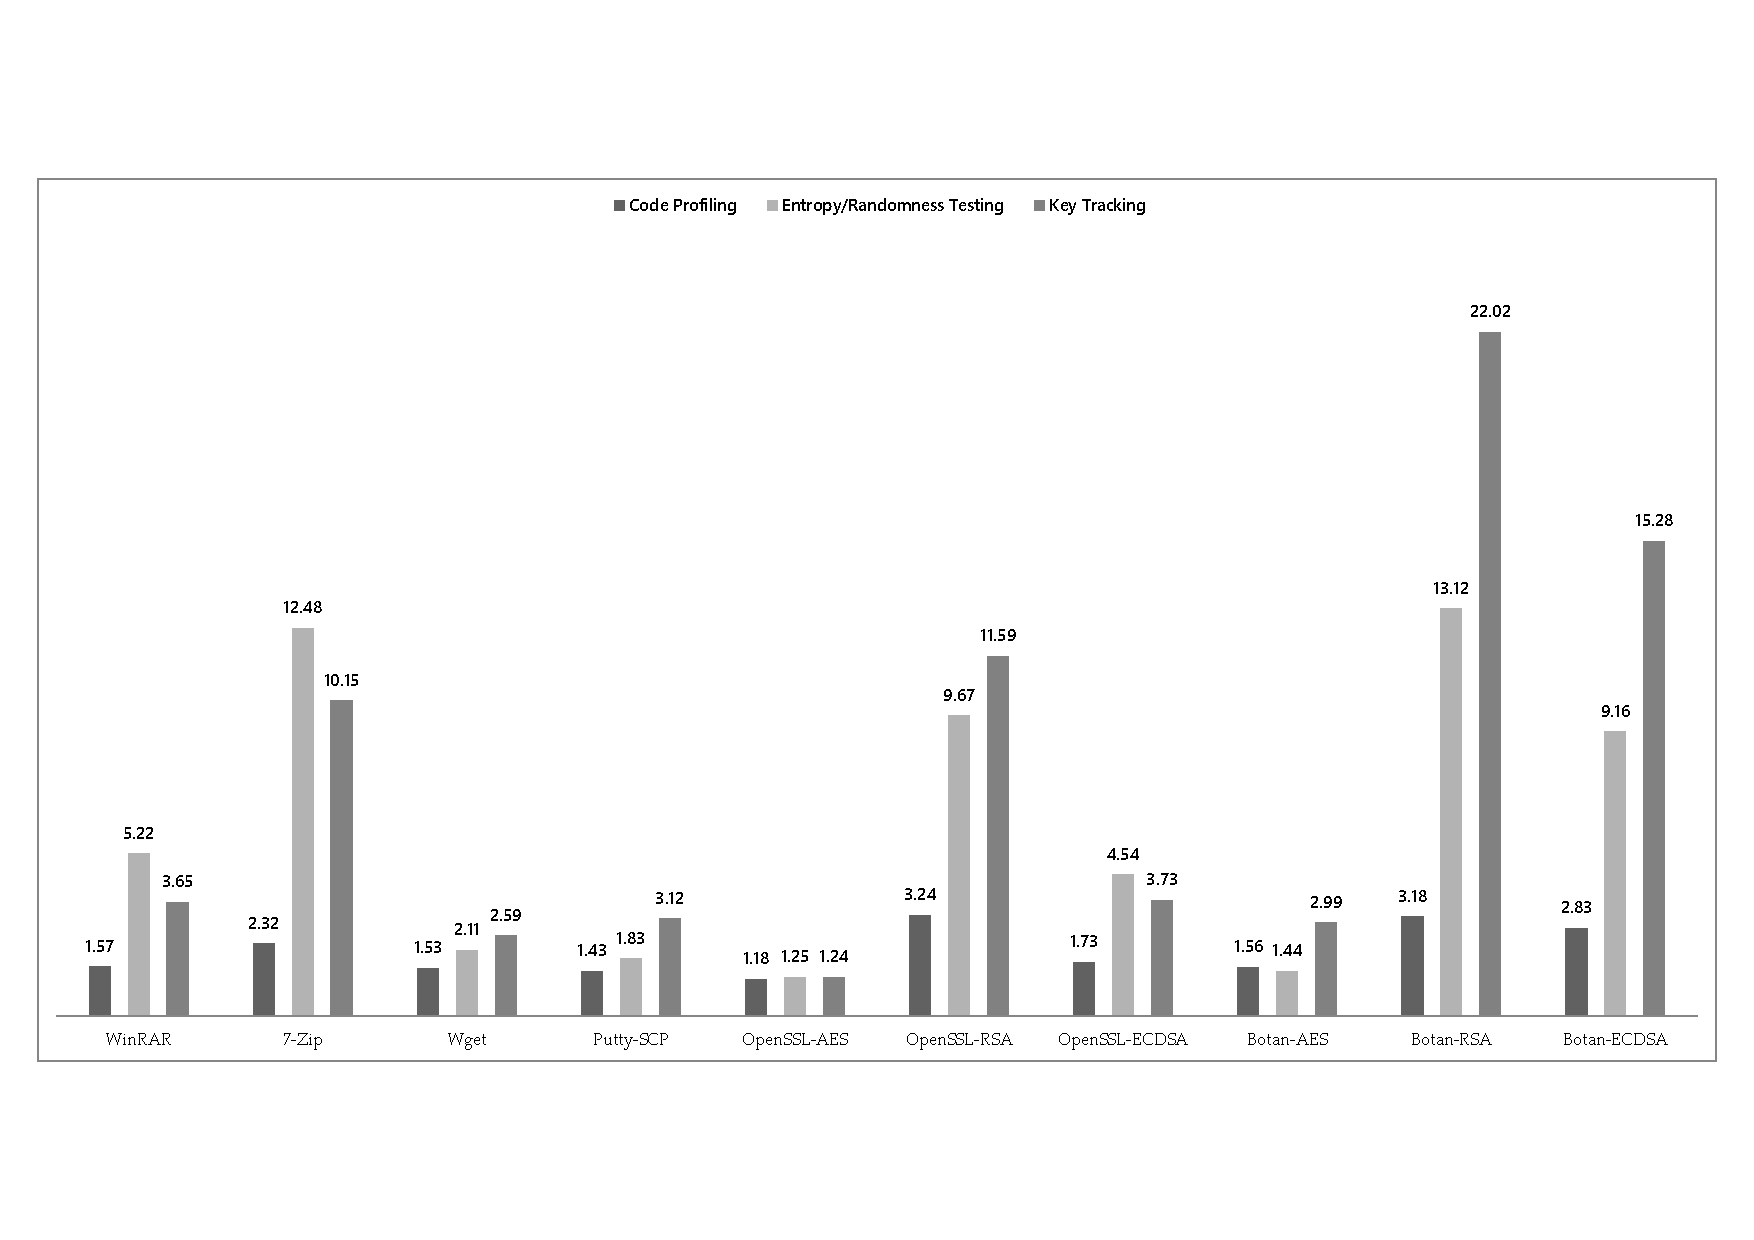
\includegraphics[width=0.5\textwidth]{barg.pdf}
% \caption{Performance overhead\label{fig:perf} }
% \end{figure}

\begin{figure*}
\centering
\resizebox{7.2in}{!}{
\includegraphics[width=1.5*\linewidth]{figure/perf.tikz}
}
\vspace{-0.1in}
\caption{Runtime overhead (times) of three pintools of \sysname compared to null PIN.}
\label{fig:spec:shadowperf}
\end{figure*}

As described in \S\ref{sec:kxray}, \sysname includes three {Pintools}: \emph{code profiling},  \emph{randomness testing}, and \emph{key tracking}. To evaluate the performance overhead of these Pintools, we selected four command-line crypto applications and two representative crypto libraries. 
% to the easier measurement (and no noise) with them. % As shown in Figure~\ref{fig:perf}.
We report the performance overhead of the three Pintools compared to null PIN by running the 6 selected programs 10 times each. As shown in \autoref{fig:spec:shadowperf},
on average the performance overhead of code profiling is 2.1 times, 5.7 times for randomness testing, and 7.6 times for key tracking. We observe that the overhead is larger for programs with complex data transformation (e.g., 7-zip), asymmetric ciphers (e.g., RSA), and digital signatures (e.g., ECDSA). Nonetheless, the performance overhead is reasonable for most programs tested by \sysname. %, and we have not attempted to aggressively optimize its performance.

% To compare the efficiency our approach,
% 	we conducted seven items of testing:
% 	1) \emph{Normal execution}: programs are executed without being analyzed;
% 	2) \emph{Null PIN}: programs are executed with PIN VM but without any instrumentation stub;
% 	3) \emph{Key Pinpointing}: programs are executed with code profiling instrumentor of \sysname;
% 	4) \emph{Key tracing}: programs are executed with code tracing instrumentor of \sysname
% 		(to conduct key tracing with execution sampling, we set the instruction recording threshold to 64);
% 	5) \emph{Dataflow tainting}: programs are executed with our modified version of \emph{libdft}~\cite{kemerlis2012libdft} based on PIN framework to support Windows program;
% 	6) \emph{Data dependency analysis}: recorded traces are analyzed offline with \sysname scripts;
% 	7) \emph{Static Symbolization}: binary executables are statically analyzed by \emph{pysymemu}~\cite{pysymemu} to generate symbolic expression for each function.
% We choose four samples: \texttt{WinRAR}, \texttt{ccrypt}, \texttt{Putty-SCP}, and \texttt{Wget} in \textsc{CryptoZoo}.
% For dynamic analysis,
% 	\texttt{WinRAR} and \texttt{ccrypt} were executed to deal with an input file of 1MB,
% 	while \texttt{Putty-SCP} and \texttt{Wget} were executed to download a 1MB file from a local Linux server.
% To evaluate the efficacy of dynamic program analysis,
%     we also set a terminating condition for each program:
%     if the overhead of one testing exceeds to 10,000 times of the original raw execution,
%     or the network connection is time out, the testing is terminated.



%We also tested the execution time of \sysname. In our experiments, \sysname successfully instrumented all test targets and finished the analysis within several minutes to several hours according to the size of the target program. The most time-consuming stage is the offline taint analysis, which consumes the execution trace and builds data dependency between the key and the inputs. As Table~\ref{tab:insecKey} shows, the size of execution trace varies from xx MB to XX GB. All of them can be recorded without affecting the normal execution of the test target.

% The lightweight key pinpointing slowed down the execution by about 50-100 times.
% The key tracing slowed down each program's execution by about 100-200 times,
% 	and programs such as \texttt{Putty-SCP} can successfully fulfilled network data transferring without suffering from time-out issue.
% By comparison,
% 	dataflow tainting, the prerequisite analysis of many existing approaches, failed to pass each test within a reasonable time.
% For the static analysis part,
% 	since our analysis only deals with the a relatively small size of recorded traces~\footnote{in column 7, size of analyzed tailored trace is listed},
% 	it achieved an average analysis speed of 0.1M/s.
% Even if our analysis tools were implemented in python scripts,
%     the analysis time was less than seven minutes for every case.
% In comparison,
% 	static symbolization methods analyzes the entire program instead of tracing data.
% For programs with moderate size (\texttt{Wget} and \texttt{Putty-SCP}),
%     it spent one or more days to accomplish the symbolization process,
%     and this does not include the latter matching procedure (which we did not implement).


